\documentclass[aspectratio=169]{beamer}
\usepackage{cmap}
\usepackage{xfrac}
\usepackage[utf8]{inputenc}
\usepackage[T2A]{fontenc}
\usepackage[russian]{babel}
\usepackage{graphicx}
\usepackage{xcolor}


\usetheme{Berlin}

\title[Моделирование количества сошедших вагонов]{Моделирование количества подвижных единиц грузового поезда в сходе с рельсов на основе метода максимального правдоподобия}
\author[Е.В.Королёв \and А.Н.Игнатов]{Работу выполнил: Королёв Егор Владимирович, студент группы М8О-401Б-18 \and Научный руководитель: Игнатов Алексей Николаевич, к.ф.-м.н., доцент}
\institute[НИУ МАИ]{Московский авиационный институт (НИУ)}

\newcommand{\norm}[1]{\left\lVert#1\right\rVert}
\definecolor{myBlue}{RGB}{0, 128, 0}
\definecolor{myGreen}{RGB}{1, 4, 255}

\begin{document}
    \begin{frame}
        \maketitle
    \end{frame}


    \section{Введение}
    \begin{frame}{Введение}
        \begin{block}{Прогресс написания ВКР}
            \begin{enumerate}
                \item написано 50 страниц;
                \item приведен предварительный анализ данных;
                \item построено 96 регрессионных моделей;
                \item написана программная реализация ММП;
            \end{enumerate}
        \end{block}
    \end{frame}

    
    \begin{frame}{Введение}
        \begin{block}{Проблема}
            В странах с большой ж/д сетью и большим потоком перемещения поездов существует проблема схода составов с рельс. Последствия схода могут привести к экологическим, экономическим и логистическим проблемам. В РФ в среднем происходит 1 авария каждые 4 дня. Поэтому проблема представляет интерес для железнодорожных компаний.
        \end{block}
    
        \begin{block}{Задача}
            Для заданного набора данных необходимо построить предсказательную модель количества сошедших подвижных единиц в составе.
        \end{block}
    \end{frame}


    \section{Предварительный анализ данных}
    \begin{frame}{Описание признаков}
        \centering
        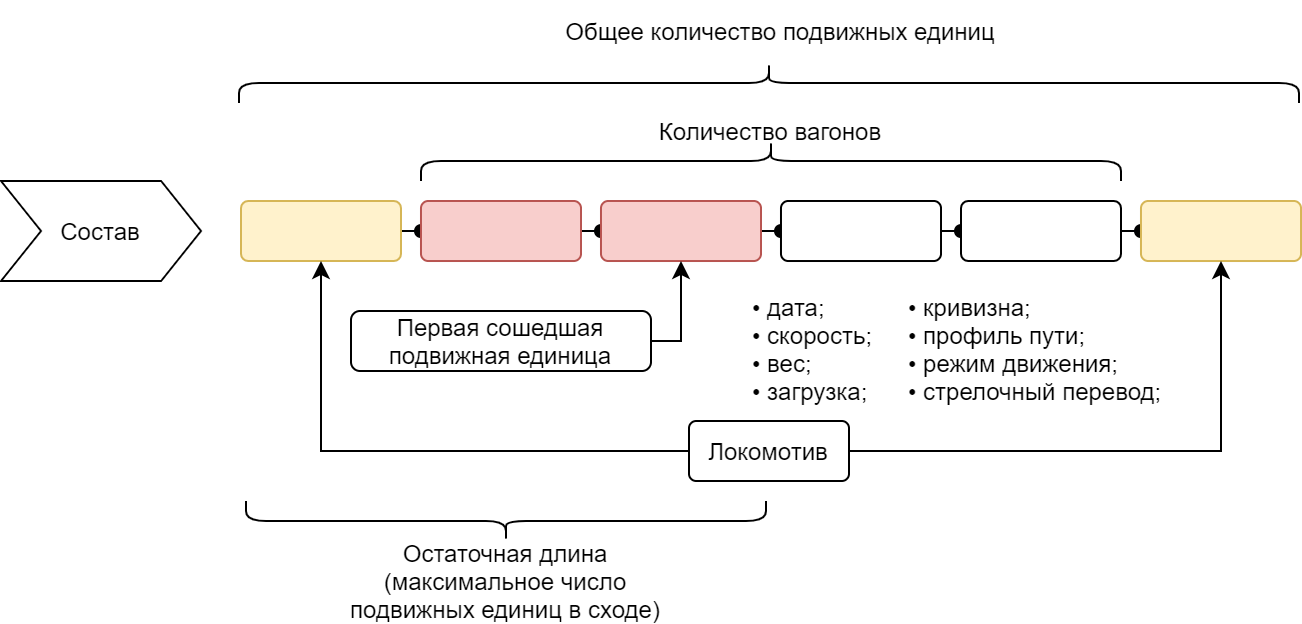
\includegraphics[width=0.8\linewidth]{src/train.png}
    \end{frame}


    \begin{frame}{Описание признаков}
        \begin{block}{Разреженность данных}
            \begin{itemize}
                \item мощность выборки $n = 56$;
                \item признак 'Режим движения' имеет $23$ пропусков ($41\%$);
                \item признак 'Профиль пути' имеет $12$ пропусков ($21\%$);
                \item признак 'Кривизна' имеет $10$ пропусков ($17\%$);
            \end{itemize}
        \end{block}
    \end{frame}


    \begin{frame}{Корреляция признаков}
        \centering
        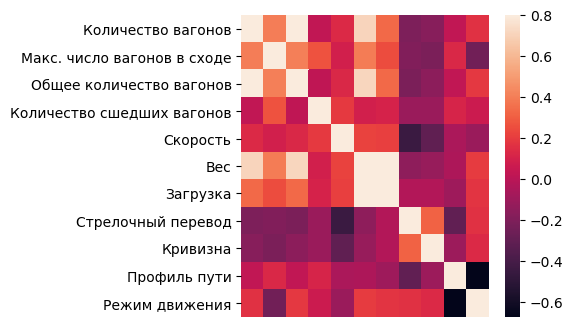
\includegraphics[width=1.3\textheight]{src/corr_plot.png}
    \end{frame}


    \begin{frame}{Конструирование признаков}
        \begin{block}{Введение новых признаков}
            \begin{itemize}
                \item $f_1 = $ профиль пути $\cdot$ макс. число вагонов в сходе;
                \item $f_2 = 1 - \frac{\text{макс. число вагонов в сходе}}{\text{общее кол-во вагонов}}$;
                \item $f_3 = $ скорость $\cdot$ загрузка;
            \end{itemize}
        \end{block}
    
        \begin{center}
            \begin{tabular}{|l|c|c|c|c|}
                \hline
                & target & $f_1$ & $f_2$ & $f_3$ \\ \hline
                target & 1.0       & 0.101375  & -0.286535 & 0.198847  \\ \hline
                $f_1$  & 0.101375  & 1.0       & -0.086693 & -0.228508 \\ \hline
                $f_2$  & -0.286535 & -0.086693 & 1.0       & -0.124420 \\ \hline
                $f_3$  & 0.198847  & -0.228508 & -0.124420 & 1.0       \\ \hline
            \end{tabular}
        \end{center}
    \end{frame}


    \begin{frame}{Оценка функции вероятности $P(\xi = x)$}
        \centering
        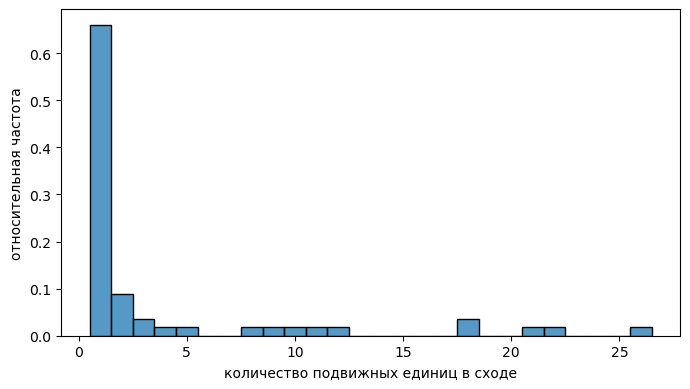
\includegraphics[width=1.3\textheight]{src/KDE.png}
    \end{frame}


    \section{Построение моделей}    
    \begin{frame}{Пуассоновская регрессия}
        \begin{block}{Функция вероятности}
            $$P(\xi = k) = \dfrac{\lambda^k}{k!}e^{-\lambda}$$
        \end{block}
        
        \begin{block}{Функция логарифмического правдоподобия}
            $$\log(L(\theta, x, y)) = \sum\limits_{i=1}^{n} \left( -\lambda(x_i, \theta) + y_i \ln(\lambda(x_i, \theta)) - \ln(y_i!) \right)$$
        \end{block}
    \end{frame}


    \begin{frame}{Определение функций $\lambda(\theta, x)$}
        \begin{enumerate}
            \item $\lambda_1(\theta, x) = e^{(\theta \cdot x)}$;
            \item $\lambda_2(\theta, x) = e^{-(\theta \cdot x)^2}$;
            \item $\lambda_3(\theta, x) = \sqrt{|5^2 - ((\theta \cdot x) - 5)^2|} + 1$;
            \item $\lambda_4(\theta, x) = ((\theta \cdot x) - 1)^2$;
            \item $\lambda_5(\theta, x) = \frac{1}{1 + (\theta \cdot x)^2}$;
            \item $\lambda_6(\theta, x) = (\theta \cdot x) (\frac{\pi}{2} + \arctan(\theta \cdot x)) + 1$;
            \item $\lambda_7(\theta, x) = \log(1 + (\theta \cdot x)^2) + 1$.
        \end{enumerate}
    \end{frame}


    \begin{frame}{Геометрическая регрессия}
        \begin{block}{Функция вероятности}
            $$P(\xi = k) = (1-p)^k p$$
        \end{block}
        
        \begin{block}{Функция логарифмического правдоподобия}
            $$\log(L(\theta, x, y)) = \sum\limits_{i = 1}^n ( y_i \ln(1 - p(x_i,\theta)) + \ln(p(x_i,\theta)) )$$
        \end{block}        
    \end{frame}

    
    \begin{frame}{Определение функций $p(\theta, x)$}
        \begin{enumerate}
            \item $p_1(\theta, x) = e^{(\theta \cdot x)}$;
            \item $p_2(\theta, x) = e^{-(\theta \cdot x)^2}$;
            \item $p_3(\theta, x) = \frac{1}{1+e^{-(\theta \cdot x)}}$;
            \item $p_4(\theta, x) = \frac{1}{1 + (\theta \cdot x)^2}$;
            \item $p_5(\theta, x) = (\theta \cdot x) (\frac{\pi}{2} + \arctan(\theta \cdot x)) + 1$.
        \end{enumerate}
    \end{frame}


    \begin{frame}{Признаковые пространства}
        \begin{enumerate}
            \item $features_1:$ (кривизна);
            \item $features_2:$ (кривизна, профиль пути);
            \item $features_3:$ (кривизна, профиль пути $\cdot$ макс. число вагонов в сходе);
            \item $features_4:$ (кривизна, $1 - \frac{\text{макс. число вагонов в сходе}}{\text{общее кол-во вагонов}}$);
            \item $features_5:$ (кривизна, профиль пути, скорость $\cdot$ загрузка);
            \item $features_6:$ (кривизна, профиль пути, скорость $\cdot$ загрузка,\\ $1 - \frac{\text{макс. число вагонов в сходе}}{\text{общее кол-во вагонов}}$);
            \item $features_7:$ (кривизна, скорость $\cdot$ загрузка, $1 - \frac{\text{макс. число вагонов в сходе}}{\text{общее кол-во вагонов}}$);
            \item $features_8:$ (скорость $\cdot$ загрузка, $1 - \frac{\text{макс. число вагонов в сходе}}{\text{общее кол-во вагонов}}$).
            \newline
        \end{enumerate}
    \end{frame}

    
    \section{Численный эксперимент}
    \begin{frame}{Программная реализация ММП}
        \begin{block}{Конструктор класса}
            \textcolor{myGreen}{def} \textcolor{myBlue}{MLM}(log\_likelihood\_fun,\\
            \begin{tabular}{p{1cm}l}
                & const\_log\_likelihood\_fun,\\
                & optim\_method, borders,\\
                & predict\_fun, param\_fun,\\
                & features, target, df)
            \end{tabular}
        \end{block}
    \end{frame}
    
    
    \begin{frame}{Численный эксперимент}
        \begin{block}{Пуассоновская регрессия}
            \begin{itemize}
                \item наилучшая модель: $(\lambda_1, features_7)$. $AIC_c = 400.13,~~\hat\theta=(0.92, -105.35, 34.34, 0.02, -2.24)$;
                \item диапазон значений: $AIC_c \sim 400.13 \div 617.6$;
            \end{itemize}
        \end{block}
    
        \begin{block}{Геометрическая регрессия}
            \begin{itemize}
                \item наилучшая модель: $(p_4, features_7)$. $AIC_c = 153.79,~~\hat\theta=(-0.68, 89.66, -113.05, -0.05, 3.31)$;
                \item диапазон значений: $AIC_c \sim 153.79 \div 352.91$;
            \end{itemize}
        \end{block}
    \end{frame}


    \section{Заключение}
    \begin{frame}{Выводы}
        \begin{block}{}
            В данной работе были построены предсказательные модели числа сошедших вагонов. Глобально их можно разделить на 2 класса: модели Пуассоновской регрессии и модели геометрической регрессии. Для каждого класса были рассмотрены различные параметрические виды и признаковые пространства.
        \end{block}
    \end{frame}

    \begin{frame}{Список литературы}
        \begin{thebibliography}{00}
            \bibitem{Ignatov:functional_dependence} Замышляев А.М., Игнатов А.Н., Кибзун А.И., Новожилов Е.О. Функциональная зависимость между количеством вагонов в сходе из-за неисправностей вагонов или пути и факторами движения // Надежность. 2018. Т. 18, № 1. С….. DOI: 10.21683/1729-2646-2018-18-1…
        \end{thebibliography}
     \end{frame}
    
    \begin{frame}{}
        \centering
        \Huge
        Спасибо за внимание!
    \end{frame}

\end{document}

